\label{sec:Wyniki}

\akapit Wyniki pomiarowe przedstawiono w poniższej tabeli. Posłużyły one do późniejszego obliczenia odpowiednich charakterystyk.

\begin{table}[H]%[htbp]
    \centering
    \caption{Zestawienie wyników pomiarów aerodynamicznych}
    \label{tab:pomiary}
    \vspace{0.6em}
    \small
    \setlength{\tabcolsep}{10pt}
    \renewcommand{\arraystretch}{1.12}
    \begin{tabular}{r r r r r r r r}
        \toprule
        $\alpha$ & $\beta$ & $N$ & $m$ & $T$ & $C$ & $n$ & $l$ \\
        \midrule
        -2.903 & 0.000 & -3.635 &  0.069 &  0.495 &  0.384 & -0.008 & -0.034 \\
        -2.000 & 0.000 & -2.908 &  0.054 &  0.524 &  0.363 & -0.009 & -0.034 \\
        -0.000 & 0.000 & -1.352 &  0.025 &  0.550 &  0.288 & -0.013 & -0.041 \\
         2.000 & 0.000 &  0.375 &  0.006 &  0.539 &  0.258 & -0.017 & -0.053 \\
         4.000 & 0.000 &  2.053 & -0.011 &  0.480 &  0.227 & -0.022 & -0.061 \\
         6.000 & 0.000 &  3.749 & -0.029 &  0.400 &  0.164 & -0.023 & -0.069 \\
         8.000 & 0.000 &  5.528 & -0.048 &  0.358 &  0.113 & -0.026 & -0.078 \\
        10.000 & 0.000 &  7.093 & -0.063 &  0.260 &  0.085 & -0.027 & -0.081 \\
        12.000 & 0.000 &  8.627 & -0.071 &  0.186 &  0.069 & -0.028 & -0.084 \\
        14.000 & 0.000 & 10.135 & -0.064 &  0.115 &  0.032 & -0.029 & -0.084 \\
        16.000 & 0.000 & 11.627 & -0.067 &  0.034 & -0.019 & -0.030 & -0.095 \\
        18.000 & 0.000 & 13.175 & -0.073 & -0.059 & -0.058 & -0.030 & -0.091 \\
        20.000 & 0.000 & 14.358 & -0.064 & -0.133 & -0.137 & -0.025 & -0.084 \\
        22.000 & 0.000 & 15.311 & -0.043 & -0.161 & -0.301 & -0.006 & -0.067 \\
        24.000 & 0.000 & 16.324 & -0.019 & -0.176 & -0.469 &  0.009 & -0.058 \\
        26.000 & 0.000 & 17.364 &  0.026 & -0.180 & -0.460 &  0.005 & -0.069 \\
        28.000 & 0.000 & 18.429 &  0.055 & -0.179 & -0.433 &  0.006 & -0.051 \\
        30.000 & 0.000 & 19.029 &  0.162 & -0.022 &  0.111 &  0.112 &  0.035 \\
        32.000 & 0.000 & 19.987 &  0.161 & -0.065 &  0.089 &  0.123 &  0.013 \\
        33.999 & 0.000 & 20.140 &  0.187 &  0.161 &  0.057 &  0.036 & -0.061 \\
        36.000 & 0.000 & 21.236 &  0.181 &  0.076 &  0.143 &  0.043 & -0.054 \\
        37.999 & 0.000 & 22.269 &  0.170 & -0.009 &  0.167 &  0.039 & -0.049 \\
        39.999 & 0.000 & 22.978 &  0.154 & -0.074 &  0.107 &  0.025 & -0.057 \\
        \bottomrule
    \end{tabular}
\end{table}

\newpage
\begin{figure}[H]
    \centering
    %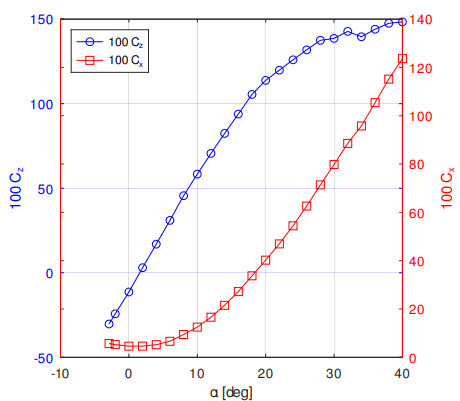
\includegraphics[width=0.5\linewidth]{zdjecia/CzCx.png}
    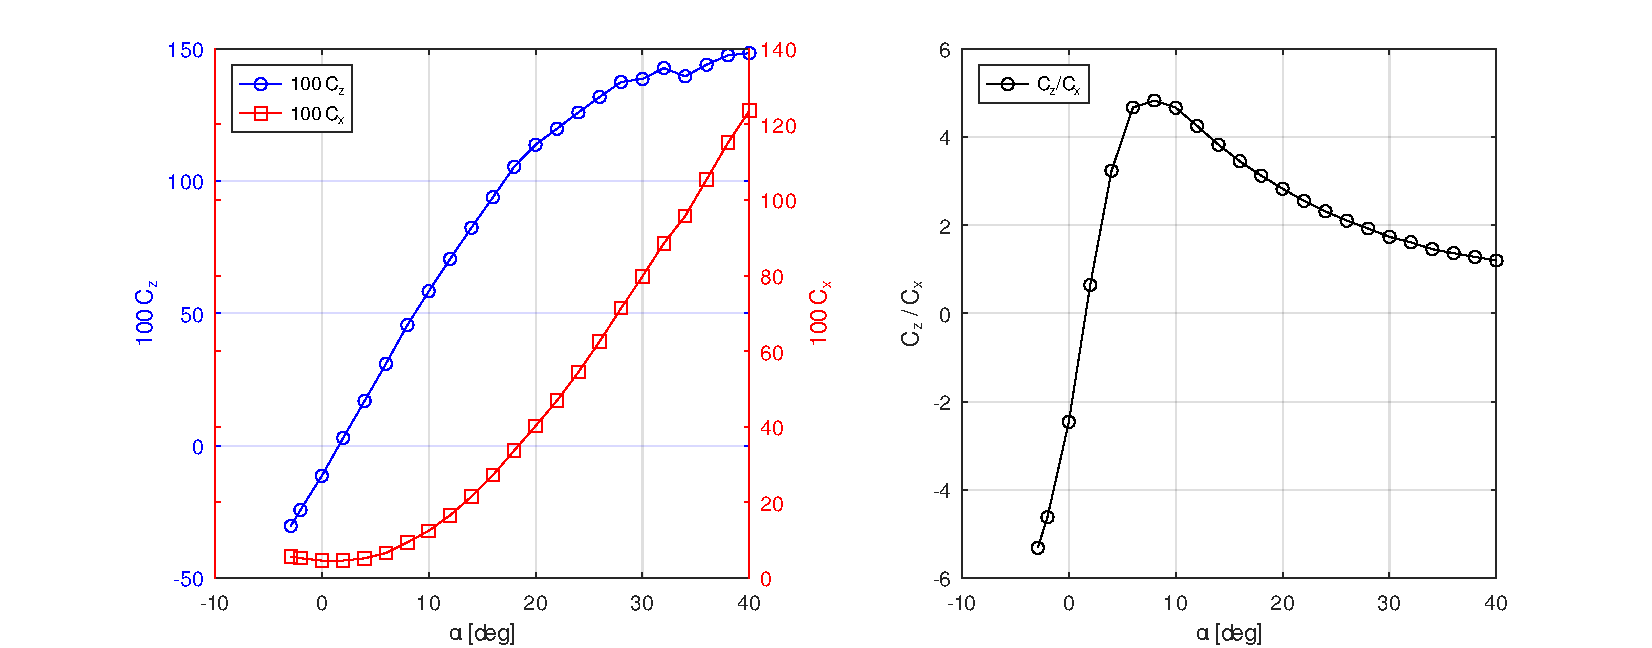
\includegraphics[width = 0.95\linewidth]{zdjecia/cz_cx_ld.pdf}
    \caption{Zależność współczynników $C_x$, $C_z$ i doskonałości $\frac{C_x}{C_z}$ od kąta natarcia skrzydła}
    \label{fig:cxcz}
\end{figure}

\begin{figure}[H]
    \centering
    %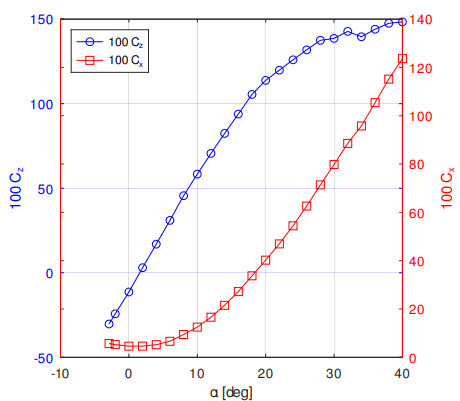
\includegraphics[width=0.5\linewidth]{zdjecia/CzCx.png}
    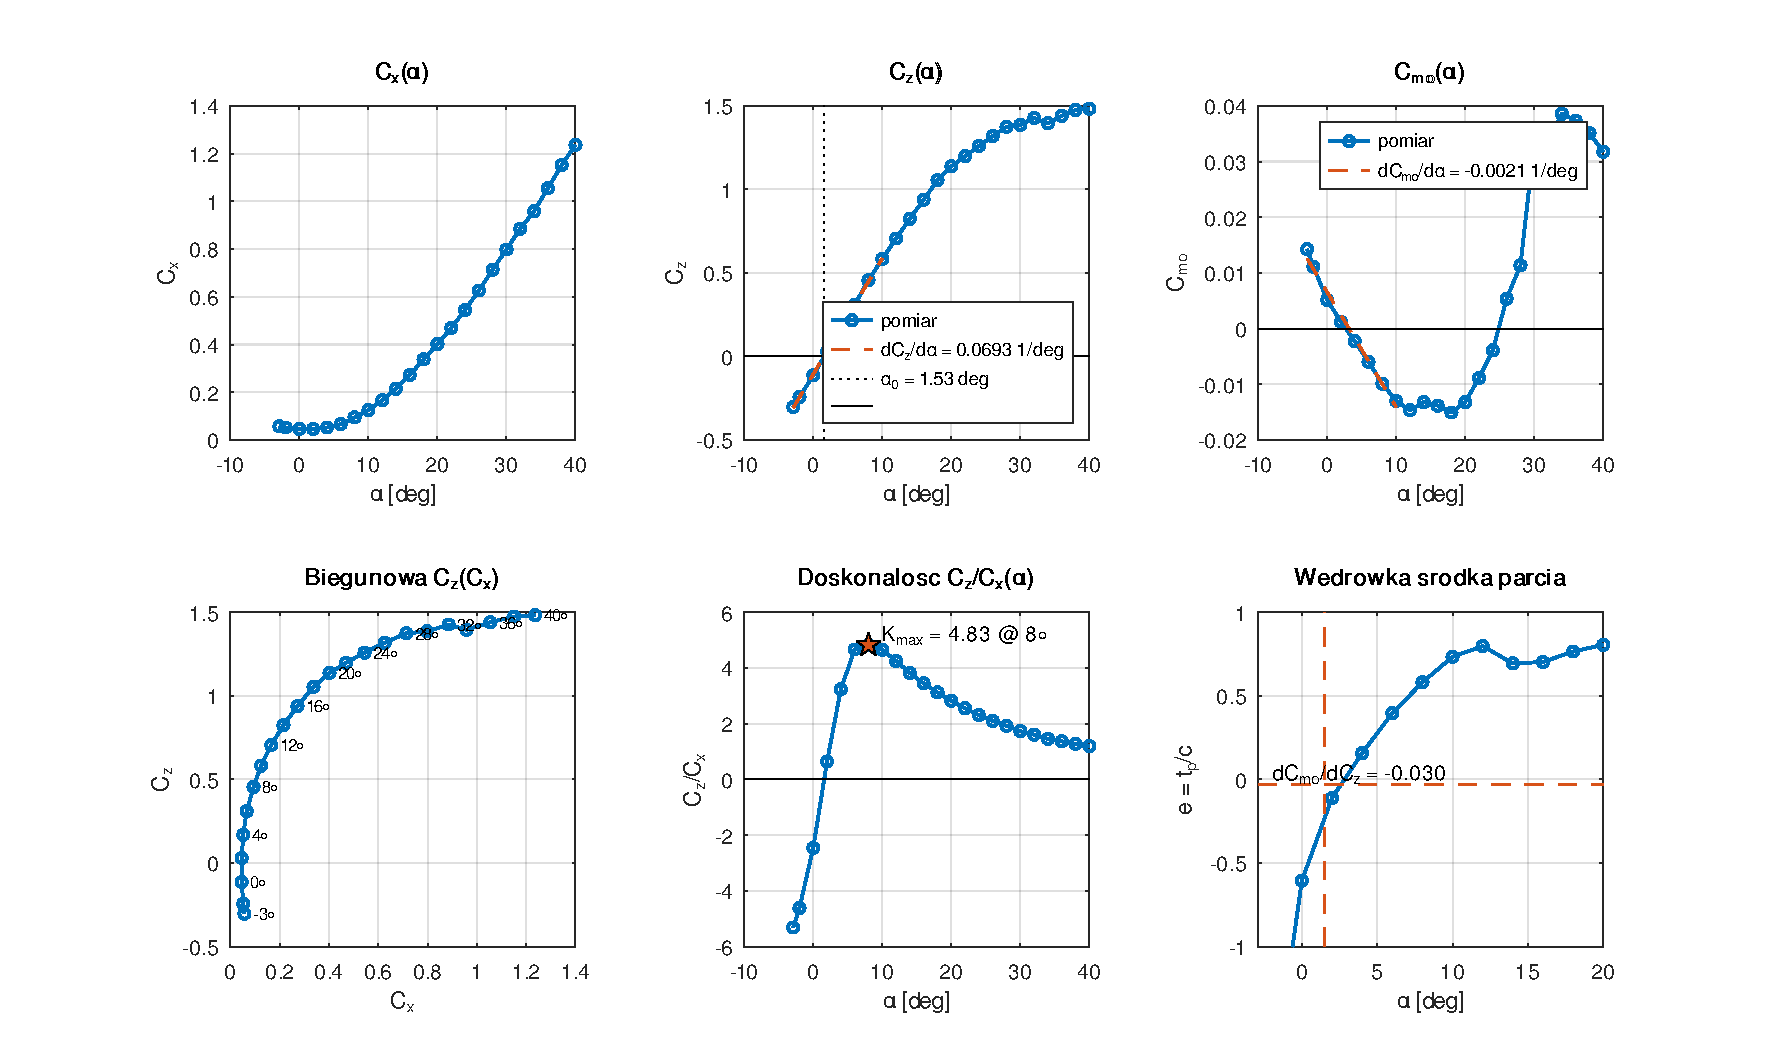
\includegraphics[width = 0.95\linewidth]{zdjecia/charakterystyki.pdf}
    \caption{Zestawienie charakterystyk na osobnych wykresach\protect\footnotemark}
    \label{fig:charakterystyki}
\end{figure}
\footnotetext{Wykres wędrówki środka parcia prawdopodobnie jest błędny}

\vfill